\documentclass[a4paper,10pt]{article}
\usepackage[utf8]{inputenc}
\usepackage{amsmath}
\usepackage{graphicx}

%opening
\title{Trouble with B-F}
\author{xxx}

\begin{document}

\maketitle

%\begin{abstract}

%\end{abstract}

\section{Simplest case}

The case we start with is the case where bound-bound transitions are basically negligible. So the statistical equlibrium equation looks like this:

\begin{equation}
 dn_i/dt = n_k T_{ki} - n_i T_{ik} = 0
\end{equation}
where $T$ denotes total rates. Now let us take the derivative of that (prime is total derivative with respect to $q_m$). 

\begin{equation}
 n_k' T_{ki} - n_i' T_{ik} + n_k T_{ki}' - n_i T_{ik}' = 0
\end{equation}
And now expand $T_{ij} = C_{ij} + R_{ij}$, and also group known quantities on the rhs and unknown ones on the lhs.
\begin{equation}
n_k' T_{ki} - n_i' T_{ik} + n_k R_{ki}' - n_i R_{ik}' = n_i C_{ik}' - n_k C_{ki}' = \Gamma_{ik}
\label{SEder}
\end{equation}
However, derivatives of radiative bound-free/free-bound rates are also known, because they are set by the background radiation field.
\begin{align}
 R_{ik} = & \int \sigma(\lambda) I(\lambda) \frac{hc}{\lambda} d\lambda \\
 R_{ki} = & \int \sigma(\lambda) (I(\lambda) + \frac{2hc^2}{\lambda^5}) \frac{hc}{\lambda}  \exp{(-hc/ \lambda k T)}  d\lambda \times  \exp{(E_i/kT)}  T^{-1.5} \times n_e \times k_{\rm Saha}
\end{align}

Which means that we can compute, first explicit dependencies of radiative rates on athmospheric parameters:
\begin{align}
 \frac{\partial R_{ik}}{\partial q_m} & = 0 \\
 \frac{\partial R_{ki}}{\partial q_m} & = .... \\
\end{align}
And then:
\begin{align}
 \frac{\partial R_{ik}}{\partial I} & = ... \\
 \frac{\partial R_{ki}}{\partial I} & = .... \\
\end{align}
And then finally put all these things together to get:
\begin{equation}
 R_{ik}' = \frac{\partial R_{ik}}{\partial q_m} + \frac{\partial R_{ik}}{\partial I} \sum_{l'} \frac{\partial I}{\partial \chi_{l'}} \frac{\partial \chi_{l'}}{\partial q_m} + 
 + \frac{\partial I}{\partial \eta_{l'}} \frac{\partial \eta_{l'}}{\partial q_m} \\
\end{equation}
We can plug this back in \ref{SEder}, to get an equation of the form:
\begin{equation}
 n_k' T_{ki} - n_i' T_{ik} =  b_i
\end{equation}
Which is then solved to obtain level responses. And this works nicely. Relative difference between finite differences and our approach is $\approx 0.1 \%$ for temperature perturbations and $\approx 0.01\%$ for pressure perturbations. Condition number of the final matrix we obtain is $\approx 10^7$.

\section{Then we include a line transition}

Now we include rather strong line. This adds both collisional and radiative terms in the above equation, but we know how to compute their derivatives. Now, this will worsen condition number ($\approx 10^9$), and agreement will be much worse, maximum discrepancies in temperature perturbations are $\approx 0.5\%$, and in density $\approx 7\%$. Decreasing the line strenght, decreases both the condition number as well as the discrepancies, down to some level where line is so weak that basically it does not matter any more if it is there or not. 

To test a more extreme case, I increased the strength of the line by additional two orders of magnitude. Condition number scaled accordingly ($\approx 10^{11}$). However, the maximum discrepancy increased only to $\approx 20\%$. Interestigly, problematic points are the ones deep in the atmosphere (see Fig.\ref{1}, corresponds to the last example).

\begin{figure}
 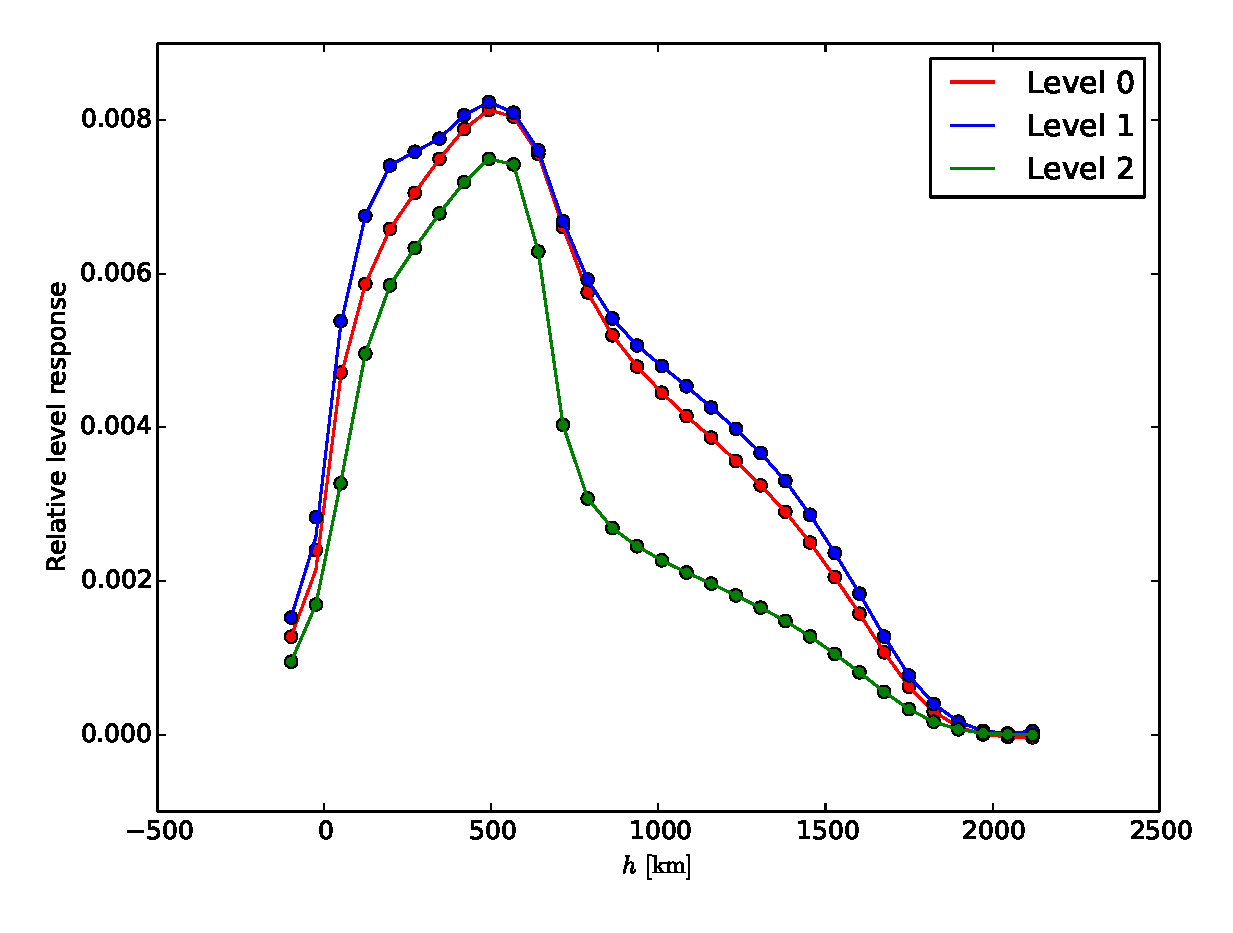
\includegraphics[width = 0.5\textwidth]{debug_local_responses_temperature.eps}
 \includegraphics[width = 0.5\textwidth]{debug_local_responses_density.eps}\\
 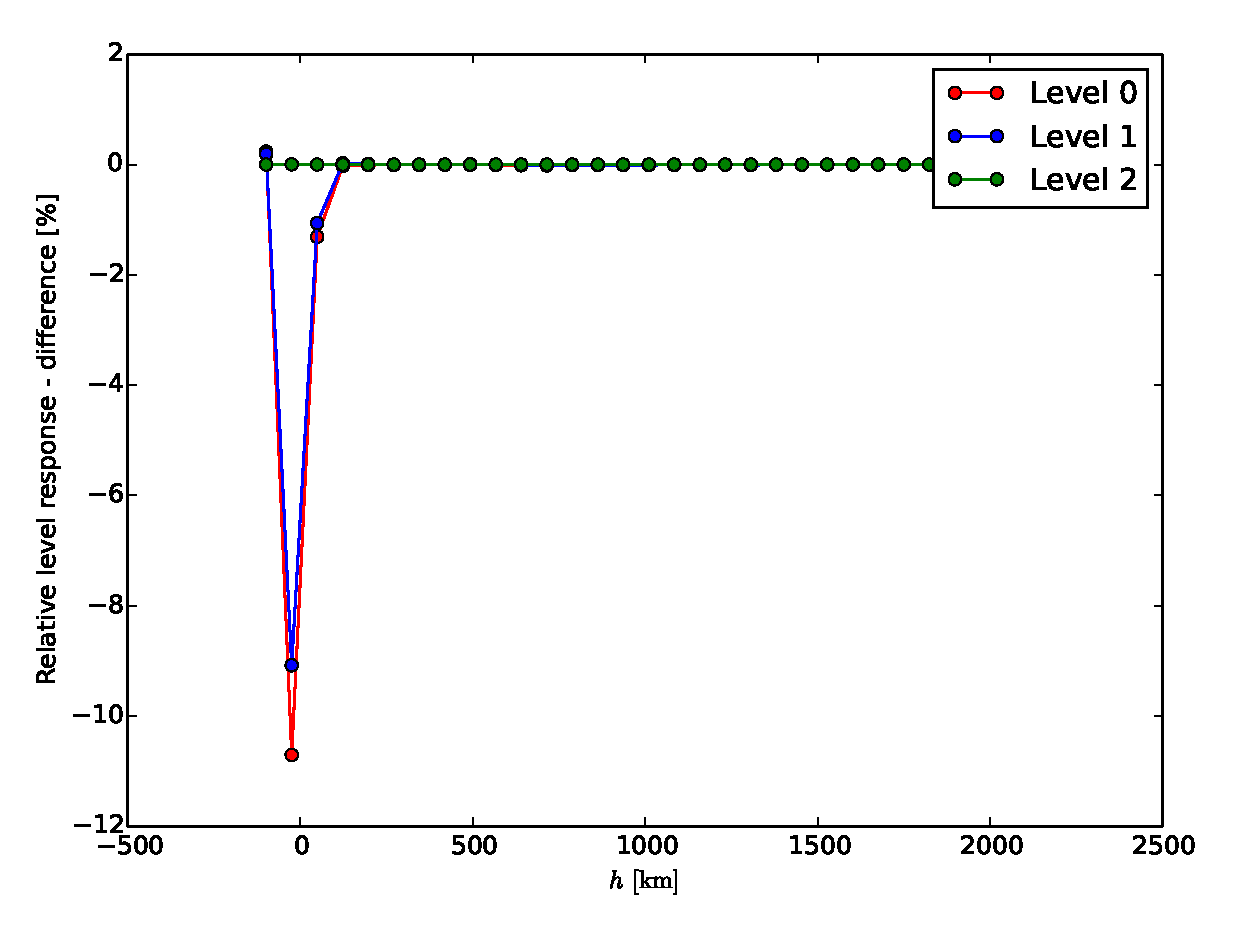
\includegraphics[width = 0.5\textwidth]{debug_local_responses_difference_temperature.eps}
 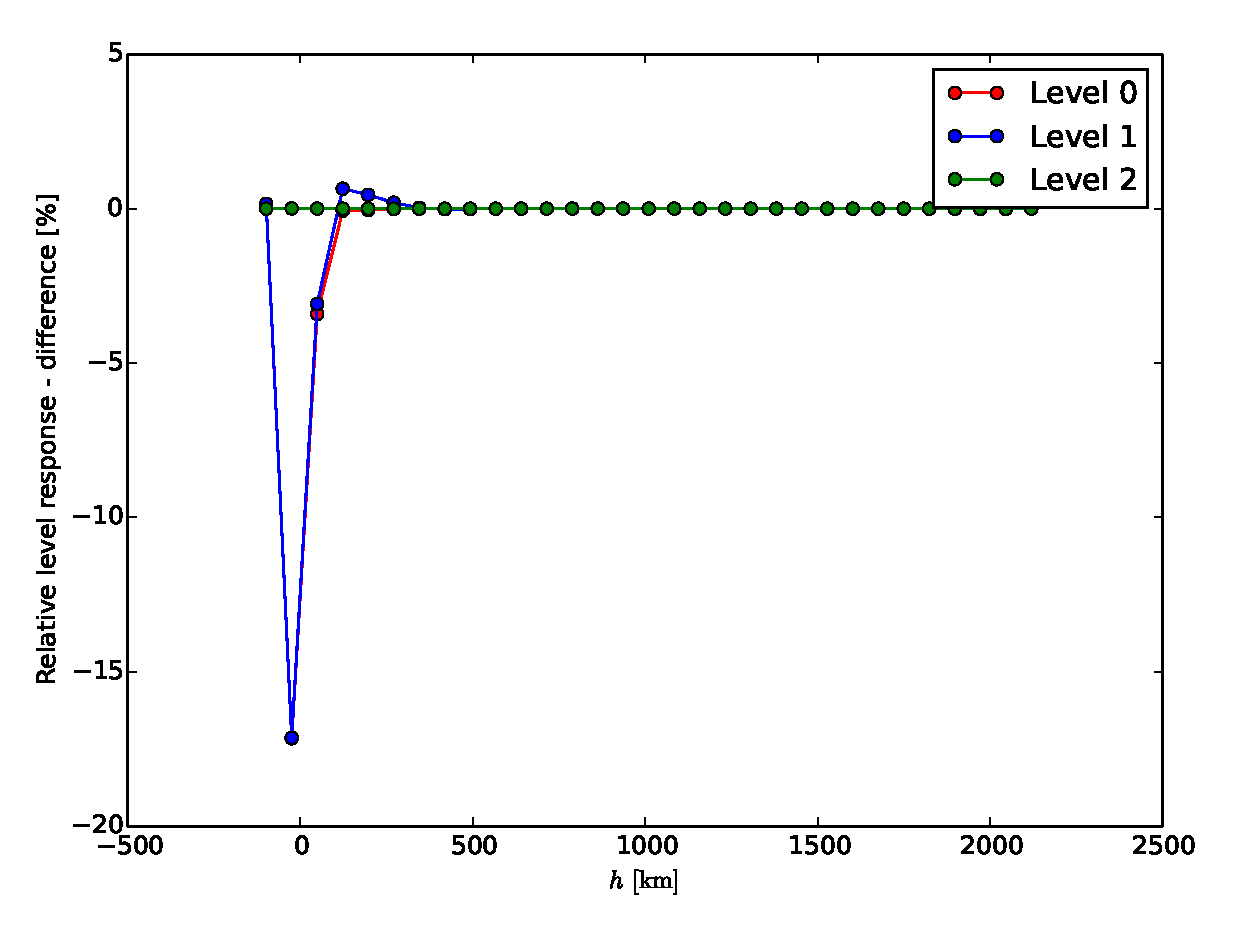
\includegraphics[width = 0.5\textwidth]{debug_local_responses_difference_density.eps}
 \caption{Upper panels are finite differences (dots), versus analytical (lines). Lower panel is relative difference between two. These are only local. Sorry for pressure responses being in linear scale :(. }
 \label{1}
\end{figure}

What is rather interesting is that choice of integration quadrature \emph{for line transition} seems to influence the thing. The magnitude of the error does not change itself by much but the particular numbers and the sign(!) of the error changes when changing the span and resolution of wavelength quadrature for the line (both for the temperature as well as density). However, at fine enough quadrature, the errors do not change much. 


\section{However, when we omit the radiative b-f transitions}

This case is baffling because system has much worse condition number, then either of those cases up there, but agreement with finite differences is very good. 
\begin{equation}
S
\end{equation}









\end{document}
